\documentclass[cameraready]{Interspeech}
\usepackage{float}
\usepackage{amsmath}
\usepackage{hyperref}
\usepackage{graphicx}
\usepackage{tabularx}
\usepackage{array}
\usepackage{booktabs}
\usepackage{dblfloatfix}

\graphicspath{{../notebooks/plots/}}

\title{Cost-Effective Predictive Modeling for Customer Targeting}

\author[affiliation={1}]{Paweł}{Pozorski}
\author[affiliation={1}]{Paweł}{Florek}
\author[affiliation={1}]{Jakub}{Półtorak}

\address{
    $^1$ Warsaw University of Technology, Poland
}

\email{\{pawel.pozorski, pawel.florek, jakub.poltorak\}.stud@pw.edu.pl}

\keywords{feature selection, profit maximization, customer targeting, ensemble methods}

\begin{document}

\maketitle

\begin{abstract}
    Abstract
\end{abstract}

\section{Introduction}

\section{Methodology}

\subsection{Problem formulation and evaluation}
\label{sec:task}

We address cost-aware customer targeting on a labelled training set $(X, y)$, where $X \in \mathbb{R}^{5000 \times 500}$ and $y$ is a roughly balanced binary response.
Each customer is assigned an acceptance probability $\hat{p} = P(y{=}1 \mid x)$; the campaign contacts the top $k \leq 1000$ customers by decreasing $\hat{p}$.
Optimisation targets a profit-oriented score rather than classification accuracy:
\[
\text{Score} = 10\,\mathrm{TP} - 5\,\mathrm{FP} - 200\,N_{\mathrm{vars}},
\]
where $N_{\mathrm{vars}}$ denotes the number of features declared in the submission.
The linear penalty on $N_{\mathrm{vars}}$ couples predictive performance with model parsimony: each additional variable requires twenty extra true positives to break even.

All design choices---feature subsets, model hyperparameters, and the contact count $k$---are estimated on training data using 5-fold stratified cross-validation.
The business scorer ranks validation-fold probabilities, computes
$\mathrm{Score}_k = 10\,\mathrm{TP}_k - 5\,\mathrm{FP}_k - 200\,N_{\mathrm{vars}}$ for $k = 1, \ldots, 1000$,
and selects the maximising $k$.
Out-of-fold (OOF) predictions aggregate held-out fold scores and are used for contact-set size selection, thereby avoiding optimistic bias from in-sample fitting.
Models are subsequently refit on the full training set prior to test-time ranking.
Under the contact cost structure, a customer is profitable in expectation iff $\hat{p} > 1/3$, since $E[\text{contact}] = 15p - 5$.

\subsection{Feature selection}
\label{sec:featsel}

Feature selection proceeds in three stages and yields a ranked shortlist together with prefix subsets \texttt{top\_01}--\texttt{top\_26} used throughout the modelling pipeline.

In \emph{Stage~1} (500 $\to$ 80 features), near-constant columns are removed by a variance threshold, then mutual information and LightGBM split-gain rankings are combined; the 80 columns with the lowest summed rank are retained.
\emph{Stage~2} (80 $\to$ 26) removes redundancy via correlation pruning ($|r| \geq 0.85$, discarding the lower-MI member of each pair) and iterative variance-inflation-factor filtering (threshold 5), followed by an $\ell_1$-regularised logistic path; the penalty parameter $C$ is chosen by cross-validated business score subject to a sparsity band of 20--30 non-zero coefficients.

\emph{Stage~3} orders the surviving features by \emph{drop-column cross-validation}.
For each feature $f$, a classifier is evaluated on all Stage-2 columns except $f$; the quantity
$\Delta_f = \text{score}_{\setminus f} - \text{score}_{\text{full}}$
quantifies the marginal profit loss attributable to $f$ (smaller $\Delta_f$ indicates higher importance).
Prefix subsets of the resulting ordering are rescored under the same metric.
Alternative importance measures (mean decrease in impurity, permutation importance, Boruta) are reported for comparison but are not used to define the primary feature order.

\subsection{Baselines}
\label{sec:baselines}

Reference models provide lower bounds on performance and verify the implementation of the business scorer; they do not enter the submission pipeline.

Dummy classifiers are fit on a zero-dimensional feature matrix ($n_{\mathrm{features}} = 0$).
The \texttt{prior} and \texttt{uniform} strategies produce constant acceptance probabilities; the \texttt{stratified} strategy yields row-wise random one-hot pseudo-probabilities.
A \texttt{RandomScoreClassifier} assigns independent $\mathrm{Uniform}(0,1)$ scores across five random seeds.
Learned references comprise logistic regression on the highest-correlation univariate predictor (\texttt{var\_389}) and on the full 500-dimensional input, the latter illustrating the effect of the feature penalty.
Supplementary experiments compare prefix subsets of ranked raw features with an equal number of PCA components, evaluated by top-$k$ F1 and ROC-AUC without the variable-cost term.

\subsection{Top-$k$ profit curve}
\label{sec:topk}

The primary modelling strategy selects a single classifier and feature subset by maximising out-of-fold profit.
Logistic regression, LightGBM, and XGBoost are compared on each prefix subset under the cross-validated business score; hyperparameters are tuned on the winning configuration using the same objective rather than ROC-AUC.
OOF acceptance probabilities are obtained by 5-fold stratified cross-validation, and the contact count is set to
$k^* = \arg\max_k \mathrm{Score}_k$ on the resulting profit curve.

\subsection{Expected-value profit targeting}
\label{sec:ev}

This approach retains the model-selection procedure of Section~\ref{sec:topk} but determines $k$ from economically motivated rules when the profit curve is flat near the contact cap.
OOF probabilities are mapped through isotonic regression prior to decision-making.
Four candidate values of $k$ are derived: (i)~a threshold walk that includes customers while $\hat{p} \geq 1/3$; (ii)~the smallest $k$ attaining at least 95\% of the peak OOF score; (iii)~the maximiser of mean fold-wise business score over a discrete grid of $k$; and (iv)~the unconstrained profit-curve maximum.
By default, the \emph{combined} rule $k = \min(k_{\mathrm{ev}}, k_{\mathrm{elbow}}, k_{\mathrm{nested}})$ is adopted.

\subsection{Rank fusion committee}
\label{sec:fusion}

We examine whether a committee of heterogeneous rankers, combined by OOF-weighted averaging, improves upon any single expert.
The committee comprises four fixed members: logistic regression on \texttt{top\_03}, LightGBM on \texttt{top\_05}, logistic regression on \texttt{top\_08}, and a Borda ranker on \texttt{top\_05} that aggregates feature-wise signed ranks into pseudo-probabilities.
Expert weights are proportional to non-negative cross-validated business scores, $w_e \propto \max(0, \text{CV business}_e)$, and the fused prediction is $\hat{p} = \sum_e w_e \hat{p}_e$.
The submission lists the union of all expert feature sets (eight variables).

\subsection{Cluster split targeting}
\label{sec:cluster}

Cluster-split targeting introduces customer heterogeneity through hard partitioning before local estimation.
For each prefix subset, the number of KMeans clusters $K \in \{2,\ldots,10\}$ is assessed via inertia and silhouette; we set $K{=}4$ after visual inspection of the diagnostic curves.
Within each cross-validation fold, features are standardised, KMeans labels are assigned, and a logistic model is fit per cluster when the training partition contains at least 80 observations; otherwise a fold-level fallback model is used.
The same feature set serves both clustering and classification.
The optimal prefix subset is selected by comparing OOF business scores across the full sweep.

\subsection{Segment-aware targeting}
\label{sec:segment}

Segment-aware targeting extends the cluster-split framework by separating the feature spaces used for segmentation and for response modelling, and by replacing KMeans with a Gaussian mixture model.
In each fold, a GMM with $K{=}5$ components is fit to scaled \texttt{top\_10} features (optionally after PCA); per-segment logistic regressions are estimated on \texttt{top\_03} only.
Variables used for segmentation are treated as latent and are excluded from the submission, which declares three features.
Pooled OOF probabilities are ranked and $k$ is chosen by the profit-curve criterion of Section~\ref{sec:topk}.

\section{Results}

\subsection{Feature selection}
\label{res:featsel}

Drop-column ranking places \texttt{var\_389} first (Table~\ref{tab:topfeat}).
The penalised cross-validated business score is maximised by \texttt{top\_01} (2\,301) and decreases monotonically with subset cardinality (\texttt{top\_26}: $-2\,684$), whereas ROC-AUC continues to increase (Table~\ref{tab:featsets}), indicating a divergence between discrimination and profit under the feature penalty.

\begin{table}[t]
    \centering
    \caption{Top-ranked features after drop-column CV (Stage~3).}
    \label{tab:topfeat}
    \small
    \begin{tabular}{cl}
        \toprule
        Rank & Feature \\
        \midrule
        1 & \texttt{var\_389} \\
        2 & \texttt{var\_308} \\
        3 & \texttt{var\_93} \\
        4 & \texttt{var\_87} \\
        5 & \texttt{var\_254} \\
        \bottomrule
    \end{tabular}
\end{table}

\begin{table}[t]
    \centering
    \caption{Stage-3 prefix subsets: 5-fold CV business score (with feature penalty) and ROC-AUC.}
    \label{tab:featsets}
    \footnotesize
    \setlength{\tabcolsep}{3pt}
    \begin{tabular}{lrrr}
        \toprule
        Subset & $N_{\mathrm{vars}}$ & CV business & ROC-AUC \\
        \midrule
        \texttt{top\_01} & 1  & \textbf{2\,301} & 0.547 \\
        \texttt{top\_03} & 3  & 1\,891 & 0.551 \\
        \texttt{top\_05} & 5  & 1\,490 & 0.590 \\
        \texttt{top\_08} & 8  & 898  & 0.583 \\
        \texttt{top\_10} & 10 & 486  & 0.617 \\
        \texttt{top\_15} & 15 & $-484$ & 0.619 \\
        \texttt{top\_20} & 20 & $-1\,472$ & 0.625 \\
        \texttt{top\_26} & 26 & $-2\,684$ & 0.627 \\
        \bottomrule
    \end{tabular}
\end{table}

\subsection{Baselines}
\label{res:baselines}

Table~\ref{tab:baselines} summarises reference scores under 5-fold cross-validation.
Dummy classifiers without declared features score approximately 2\,475 at $k{=}1000$, consistent with the class prior under a balanced sample.
Logistic regression on \texttt{var\_389} attains 2\,301 and therefore falls below the no-skill floor once the single-feature penalty is applied.
With all 500 variables declared, the best-tuned logistic model yields $-97\,493$ despite F1~$\approx 0.668$; the corresponding OOF profit curve is shown in Appendix~\ref{fig:baseline}.

\begin{table}[t]
    \centering
    \caption{Reference baseline scores (5-fold CV, with feature penalty).}
    \label{tab:baselines}
    \small
    \begin{tabular}{lrrr}
        \toprule
        Baseline & Features & Business & F1@top-$k$ \\
        \midrule
        Prior / uniform dummy & 0 & 2\,475 & 0.666 \\
        Stratified dummy      & 0 & 2\,474 & 0.665 \\
        Random ranker (mean)  & 0 & 2\,475 & 0.665 \\
        Logistic (\texttt{var\_389}) & 1 & 2\,301 & 0.668 \\
        Logistic (500 feat.)  & 500 & $-97\,493$ & 0.668 \\
        \bottomrule
    \end{tabular}
\end{table}

A supplementary comparison contrasts prefix subsets of Stage-3 ranked raw features with an equal number of PCA components (all 500 columns scaled; 25 components fit once).
The same logistic penalty $C$ as the best 500-feature baseline is used.
Table~\ref{tab:pca_raw} reports top-$k$ F1 and ROC-AUC only---no business score or feature penalty, since PCA dimensions are not submission variables.
Raw ranked features achieve equal or higher F1 at every $k$; PCA attains slightly higher ROC-AUC only at $k{=}5$ and $k{=}10$, but not at $k{=}25$.
This might indicate that more features introduce noise.

\begin{table}[t]
    \centering
    \caption{Top-$k$ raw ranked features vs.\ PCA components (5-fold CV logistic regression).}
    \label{tab:pca_raw}
    \footnotesize
    \setlength{\tabcolsep}{4pt}
    \begin{tabular}{crrrr}
        \toprule
        $k$ & F1 raw & F1 PCA & ROC-AUC raw & ROC-AUC PCA \\
        \midrule
        1  & \textbf{0.668} & 0.666 & 0.555 & 0.555 \\
        3  & \textbf{0.669} & 0.665 & 0.570 & 0.584 \\
        5  & \textbf{0.669} & 0.665 & 0.581 & 0.591 \\
        10 & \textbf{0.669} & 0.666 & 0.594 & 0.598 \\
        15 & \textbf{0.670} & 0.667 & 0.597 & 0.599 \\
        25 & \textbf{0.670} & 0.667 & 0.603 & 0.598 \\
        \bottomrule
    \end{tabular}
\end{table}

\subsection{Top-$k$ profit curve}
\label{res:topk}

Among the candidate model families, logistic regression on \texttt{var\_389} achieves the highest cross-validated business score (2\,301; $C{=}0.001$ after hyperparameter tuning).
The OOF profit curve peaks at $k{=}997$ with score 3\,290 (565~TP, 432~FP; Table~\ref{tab:oof}, Appendix~\ref{fig:topk}).
Tree-based models and enlarged feature subsets fail to improve the penalised objective.


\subsection{Rank fusion}
\label{res:fusion}

The weighted committee attains an OOF score of 2\,085 at $k{=}994$ when eight features are declared.
Although true positives increase to 577 relative to the single-expert logistic model, probability averaging degrades ranking at the head of the list; see Appendix~\ref{fig:fusion}.

\begin{figure*}[t!]
    \centering
    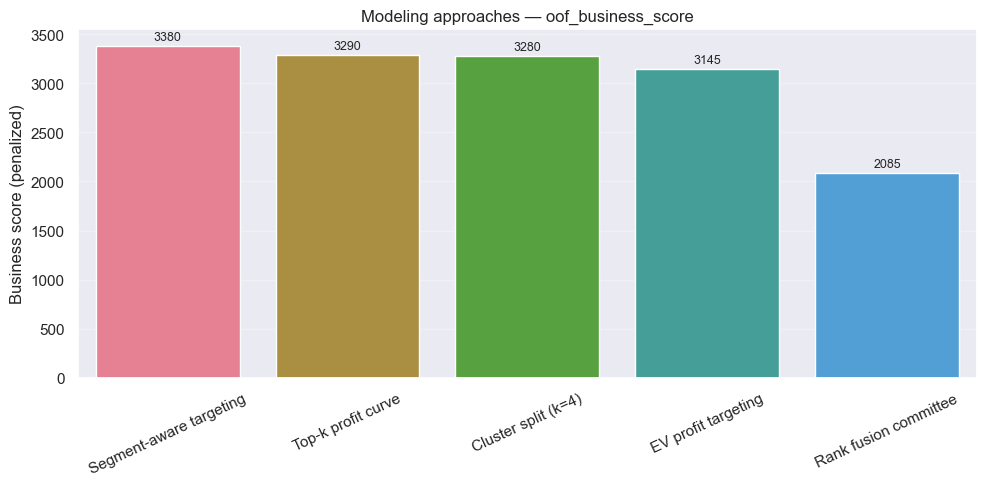
\includegraphics[width=0.8\textwidth]{methods_comparison.png}
    \caption{OOF business score across modelling approaches.}
    \label{fig:methods}
\end{figure*}

\subsection{Cluster split}
\label{res:cluster}

Table~\ref{tab:cluster} reports the cluster-split sweep at $K{=}4$.
The best configuration uses \texttt{top\_05} (OOF 3\,280 at $k{=}998$; five features).
Enlarging the feature set beyond \texttt{top\_05} reduces OOF performance; diagnostic plots appear in Appendix~\ref{fig:cluster_k}--\ref{fig:cluster}.

\begin{table}[t]
    \centering
    \caption{Cluster-split OOF business score by prefix subset ($K{=}4$).}
    \label{tab:cluster}
    \small
    \begin{tabular}{lrr}
        \toprule
        Subset & $k$ & OOF score \\
        \midrule
        \texttt{top\_05}  & 998 & \textbf{3\,280} \\
        \texttt{top\_03}   & 996 & 2\,880 \\
        \texttt{top\_01}   & 999 & 2\,800 \\
        \texttt{top\_04}   & 1\,000 & 2\,660 \\
        \texttt{top\_08}   & 1\,000 & 2\,370 \\
        \texttt{top\_10}  & 999 & 2\,260 \\
        \texttt{top\_26}  & 996 & $-895$ \\
        \bottomrule
    \end{tabular}
\end{table}

\subsection{Segment-aware targeting}
\label{res:segment}

Segment-aware targeting attains the highest OOF score in the classic pipeline---3\,380 at $k{=}998$ (598~TP, 400~FP) with three declared features (Table~\ref{tab:oof}, Appendix~\ref{fig:segment}).
Relative to cluster split, the confusion counts are marginally less favourable, yet the reduction of two submitted variables ($-400$ penalty) produces a net gain of 100 points.

\subsection{Approach comparison}
\label{res:compare}



Table~\ref{tab:oof} and Figure~\ref{fig:methods} aggregate performance across the five modelling strategies.
Segment-aware targeting occupies the first rank; rank fusion occupies the last.

\begin{table}[t]
    \centering
    \caption{OOF results by modelling approach (classic pipeline).}
    \label{tab:oof}
    \small
    \begin{tabular}{lrrrrr}
        \toprule
        Approach & Feat. & $k$ & TP & FP & OOF score \\
        \midrule
        Segment targeting  & 3 & 998 & 598 & 400 & \textbf{3\,380} \\
        Top-$k$ profit curve & 1 & 997 & 565 & 432 & 3\,290 \\
        Cluster split      & 5 & 998 & 618 & 380 & 3\,280 \\
        EV targeting       & 1 & 939 & 536 & 403 & 3\,145 \\
        Rank fusion        & 8 & 994 & 577 & 417 & 2\,085 \\
        \bottomrule
    \end{tabular}
\end{table}

\section{Conclusions}

The experiments indicate that profit-aligned feature selection is a prerequisite for competitive performance: \texttt{var\_389} dominates Stage-3 subsets, and additional variables reduce the business score despite gains in ROC-AUC.
Segment-aware targeting achieves the most favourable balance between OOF profit (3\,380) and feature parsimony (three variables). More features means more penalty, which degrades the performance of the committee, but might also introduce more noise (PCA analysis) as F1 did not improve.

\section{AI Disclosure}
This report was edited with AI assistance, to improve clarity, consistency, and formatting. Part of the docstrings, some phrasing and code refactoring or debugging were refined using AI tools, but all scientific decisions and interpretations are the authors' own. The core content, experimental design, and analysis were developed by the authors.

\newpage
\appendix

\section{Supplementary figures}

\begin{figure}[h]
    \centering
    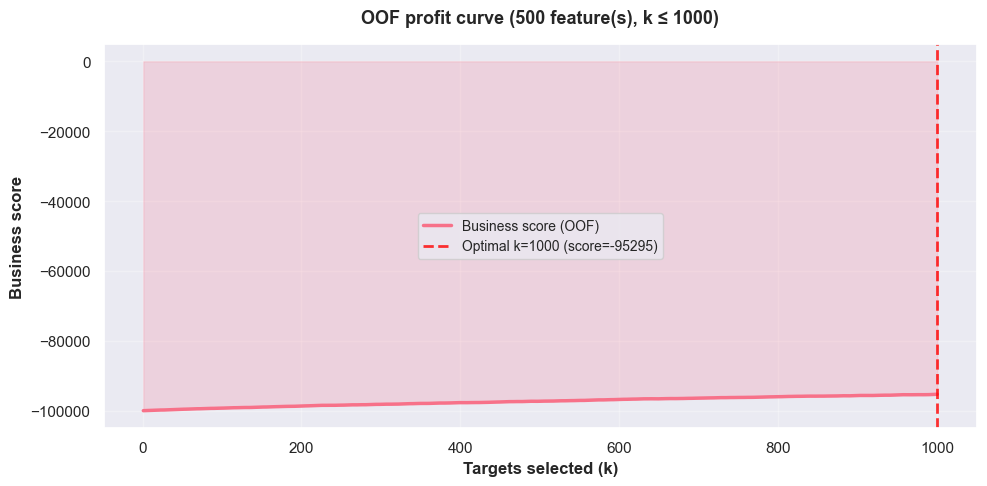
\includegraphics[width=\linewidth]{baseline_profit_curve.png}
    \caption{OOF profit curve for 500-feature logistic regression (TP\,=\,647 at $k{=}1000$, score $-95\,295$).}
    \label{fig:baseline}
\end{figure}

\begin{figure}[h]
    \centering
    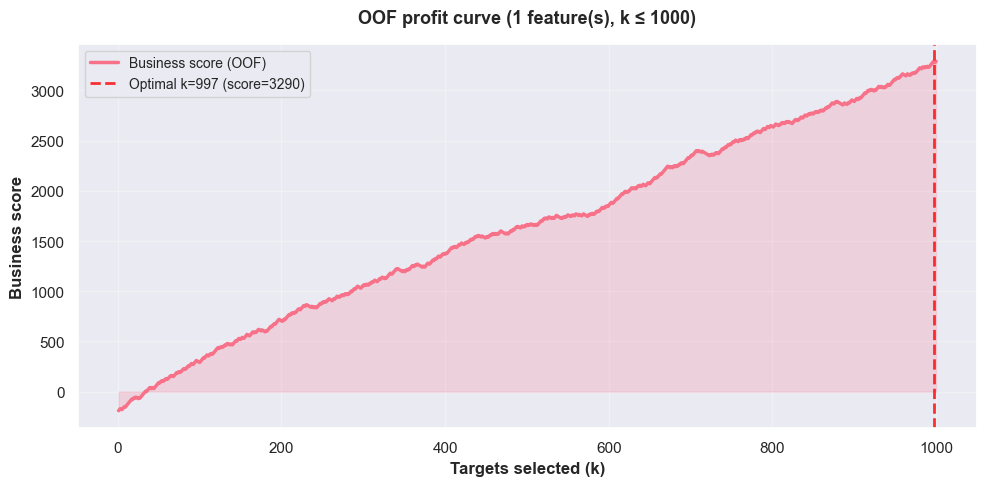
\includegraphics[width=\linewidth]{topk_profit_curve.png}
    \caption{Top-$k$ profit curve: logistic regression on \texttt{var\_389} ($k{=}997$, OOF 3\,290).}
    \label{fig:topk}
\end{figure}

\begin{figure}[h]
    \centering
    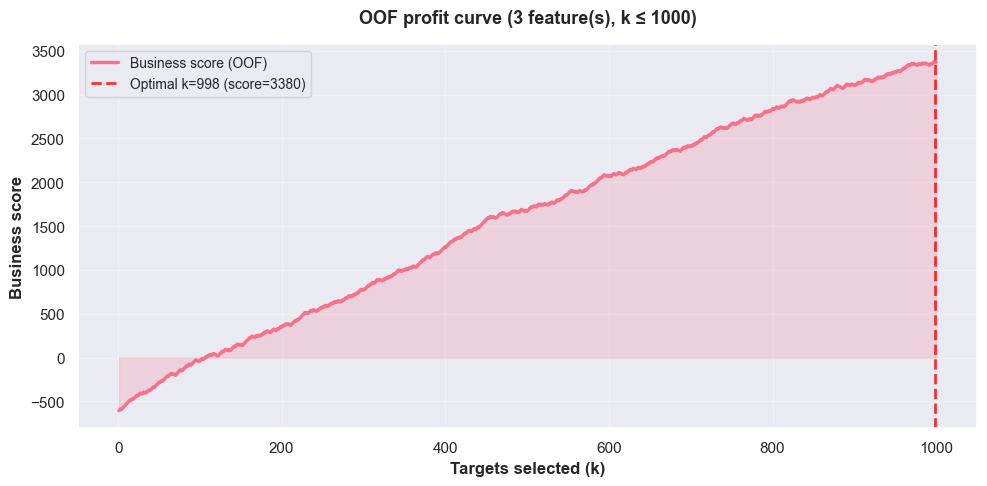
\includegraphics[width=\linewidth]{segment_targeting_profit_curve.png}
    \caption{Segment-aware targeting OOF profit curve ($k{=}998$, OOF 3\,380).}
    \label{fig:segment}
\end{figure}

\begin{figure}[h]
    \centering
    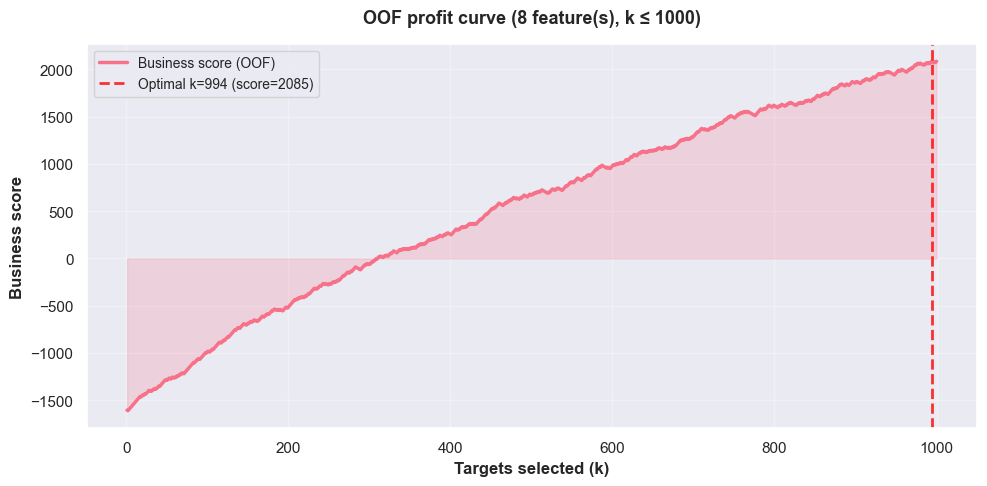
\includegraphics[width=\linewidth]{rank_fusion_profit_curve.png}
    \caption{Rank fusion committee OOF profit curve (OOF 2\,085, eight features).}
    \label{fig:fusion}
\end{figure}

\begin{figure}[h]
    \centering
    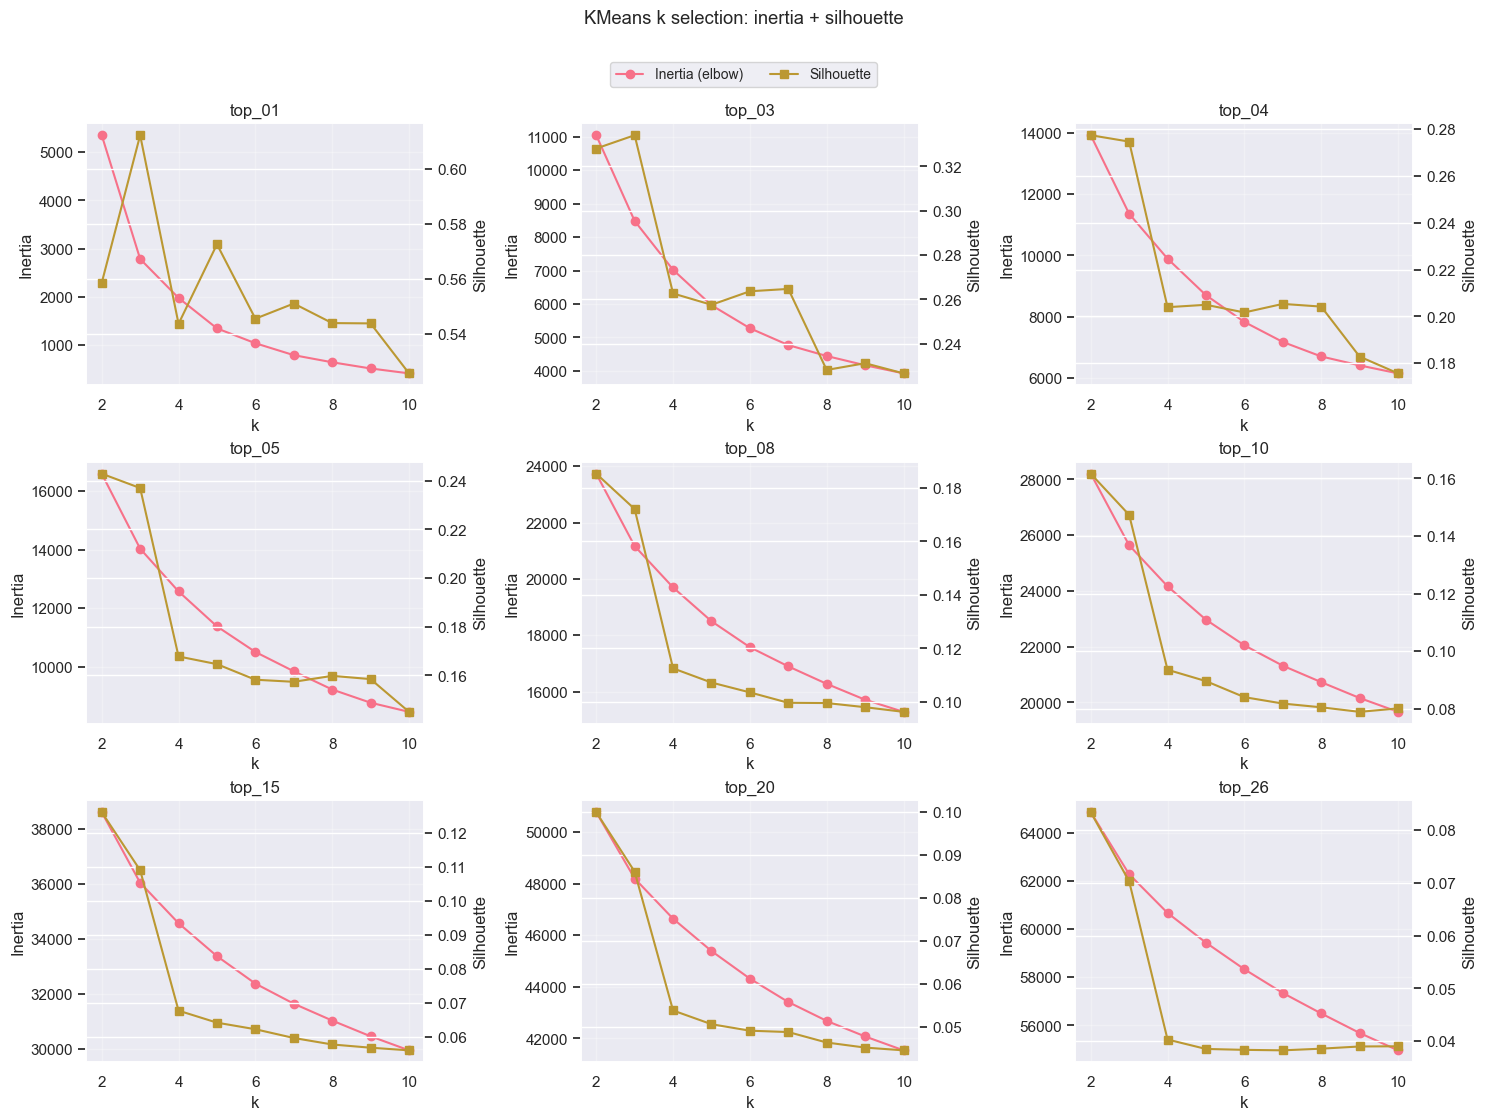
\includegraphics[width=\linewidth]{cluster_split_k_selection.png}
    \caption{KMeans diagnostics (inertia and silhouette) for cluster split.}
    \label{fig:cluster_k}
\end{figure}

\begin{figure}[h]
    \centering
    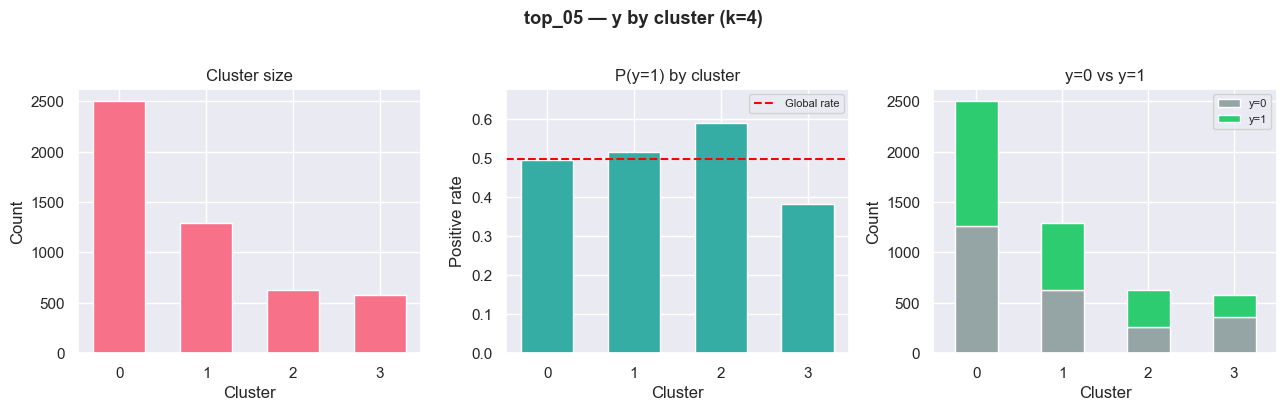
\includegraphics[width=0.48\linewidth]{cluster_split_top5_overview.png}
    \hfill
    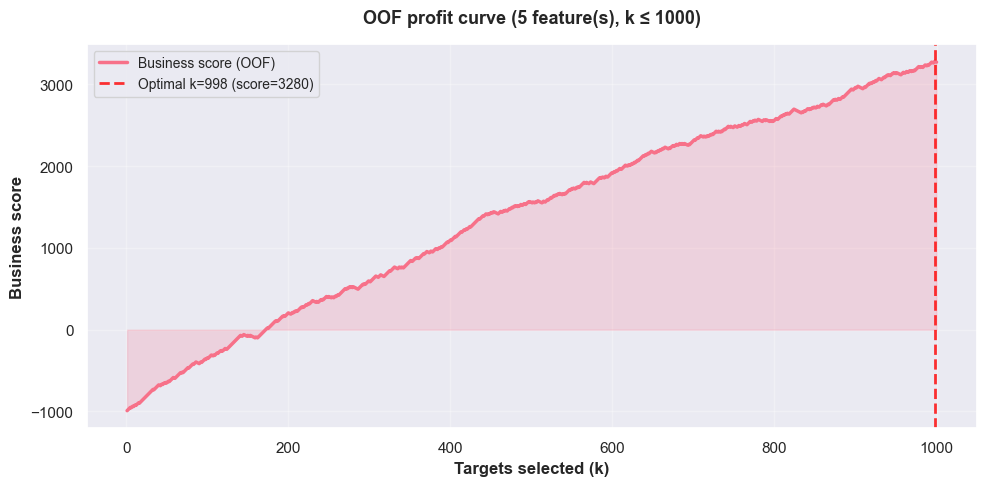
\includegraphics[width=0.48\linewidth]{cluster_split_profit_curve.png}
    \caption{Cluster split on \texttt{top\_05}: cluster overview (left) and OOF profit curve (right, score 3\,280).}
    \label{fig:cluster}
\end{figure}

\begin{figure}[h]
    \centering
    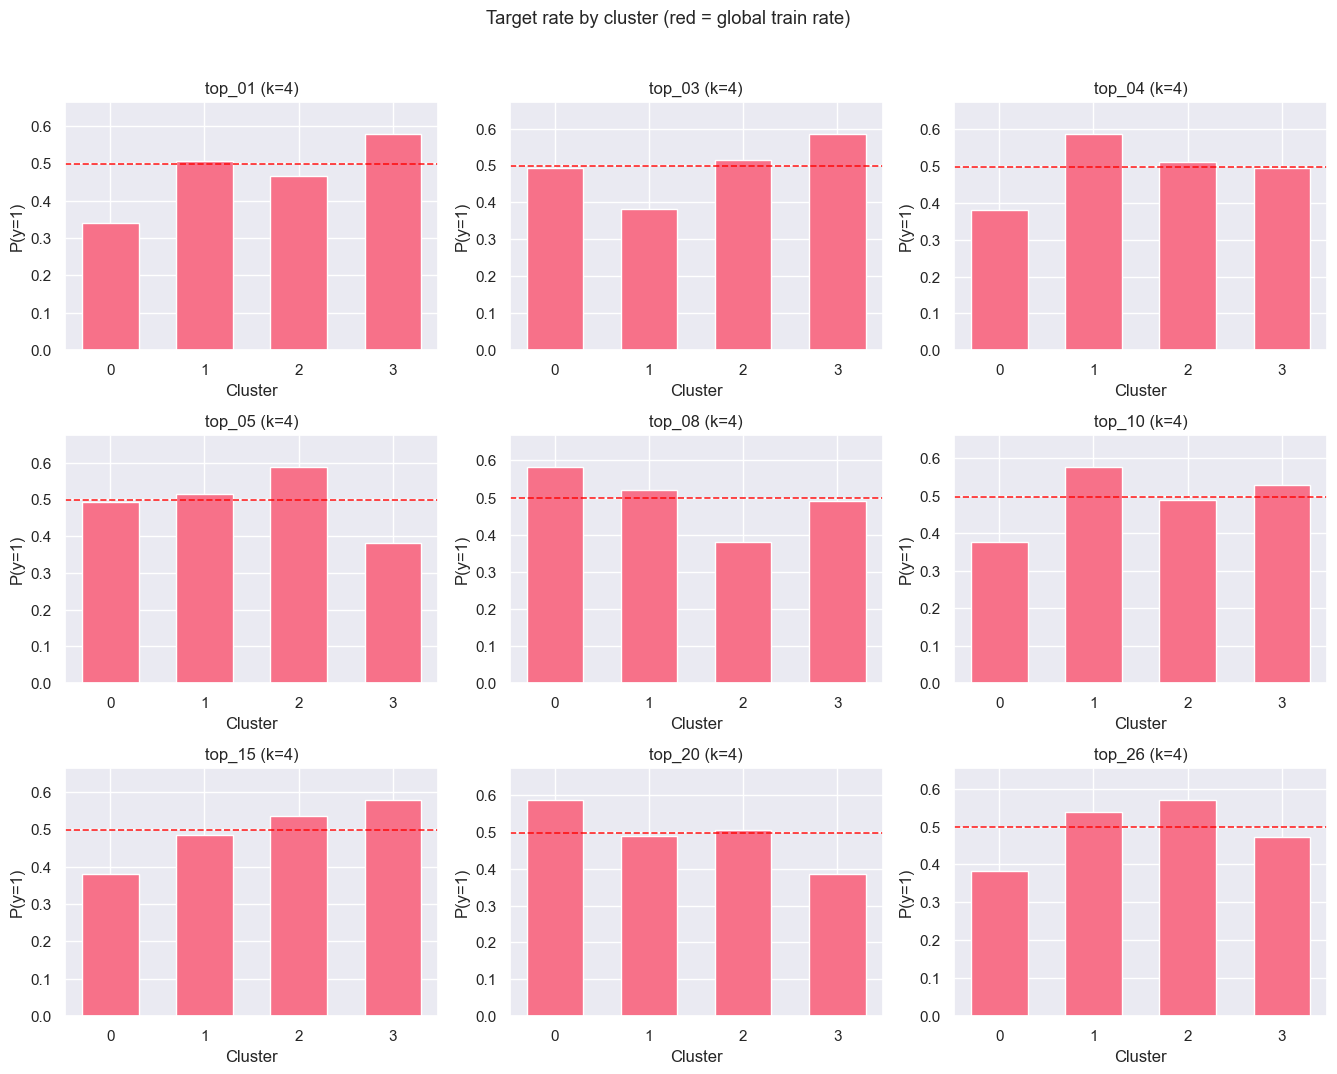
\includegraphics[width=\linewidth]{cluster_split_clusters_overview.png}
    \caption{Cluster split: per-cluster positive-rate profiles.}
    \label{fig:cluster_y}
\end{figure}

\end{document}
